\documentclass[a4paper,10pt]{report}
\usepackage[latin1]{inputenc}
\usepackage{amsmath}
\usepackage{amsmath,bm}
\usepackage{amsthm}
\usepackage{mathtools}
\usepackage{amsfonts}
\usepackage{amssymb}
\usepackage{graphicx}
\usepackage{array}
\usepackage{booktabs}
\usepackage{hyperref}
\usepackage{multicol}
\usepackage{makecell}
\usepackage[margin=0.5in]{geometry}
\usepackage[framemethod=tikz]{mdframed}
\newcommand{\myvec}[1]{\ensuremath{\begin{pmatrix}#1\end{pmatrix}}}
\let\vec\mathbf
\newcommand{\mydet}[1]{\ensuremath{\begin{vmatrix}#1\end{vmatrix}}}
\providecommand{\mbf}{\mathbf}
\providecommand{\pr}[1]{\ensuremath{\Pr\left(#1\right)}}
\providecommand{\qfunc}[1]{\ensuremath{Q\left(#1\right)}}
\providecommand{\sbrak}[1]{\ensuremath{{}\left[#1\right]}}
\providecommand{\lsbrak}[1]{\ensuremath{{}\left[#1\right.}}
\providecommand{\rsbrak}[1]{\ensuremath{{}\left.#1\right]}}
\providecommand{\brak}[1]{\ensuremath{\left(#1\right)}}
\providecommand{\lbrak}[1]{\ensuremath{\left(#1\right.}}
\providecommand{\rbrak}[1]{\ensuremath{\left.#1\right)}}
\providecommand{\cbrak}[1]{\ensuremath{\left\{#1\right\}}}
\providecommand{\lcbrak}[1]{\ensuremath{\left\{#1\right.}}
\providecommand{\rcbrak}[1]{\ensuremath{\left.#1\right\}}}
\begin{document}\raggedright{
\includegraphics[scale=0.03]{logo.png}}\hspace{12.425cm}\raggedleft FWC22037\vspace{2mm}\\
\centering\Large\textbf{ASSIGNMENT-MATRICES}\vspace{5mm}
\begin{multicols}{2}
\centering \large\textsc{C}\footnotesize\textsc{ONTENTS}\vspace{5mm}\\
\raggedright\large\textbf{1\hspace{1cm}Problem}\hspace{5.2cm}1\vspace{5mm}\\
\raggedright\large\textbf{2\hspace{1cm}Solution}\hspace{5.25cm}1\vspace{5mm}\\
\raggedright\large\textbf{3\hspace{1cm}Construction}\hspace{4.25cm}2\vspace{5mm}\\
\centering \large\textsc{1  P}\footnotesize\textsc{ROBLEM}\vspace{5mm}\\
\raggedright\large{The circle $$ x^{2}+y^{2}-4x-4y+4=0 $$ is inscribed in a triangle which has two of its sides along the co-ordinate axes.The locus of the circumcenter of the triangle is $$ x+y-xy+k(x^{2}+y^{2})^{1/2}=0 $$ Find k.}\vspace{5mm}\\
\centering \large\textsc{2  S}\footnotesize\textsc{OLUTION}\vspace{5mm}\\
\raggedright\large{1. It is given that the two sides of the triangle are the coordinate axes and the third side is \\
${\frac{x}{a}}+{\frac{y}{b}} = 1 $ can be represented as 
\begin{align}
\vec{n}^{\top}\vec{x} = C \\
\myvec{\frac{1}{a}&\frac{1}{b}}\vec{x} = 1
\end{align} }\vspace{2mm}\\
2.The circle equation is given as $$ x^{2}+y^{2}-4x-4y+4=0$$
so the center of the circle will be 
\begin{align}
\vec{c} = \myvec{2\\2}
\end{align} 
3. The distance of the point c to the line is '2'.
\begin{align}
\vec{d} =  \frac{|\vec{n}^{\top}-c|}{\vec{\|n\|}}
\end{align}
\raggedright from equation 2
\begin{gather*}
\vec{\|n\|} = \sqrt{\vec{n}^{\top} \vec{n}} \\
\vec{\|n\|} = \sqrt{\myvec{\frac{1}{a}&\frac{1}{b}}\myvec{\frac{1}{a}\\ \frac{1}{b}}}
\end{gather*}
\begin{align}
\vec{\|n\|} = \sqrt{\frac{1}{{a}^{2}} + \frac{1}{{b}^{2}}}
\end{align}
Distance of point \textbf{p} to the line(2) is
\begin{align*}
2 = \frac{\myvec{\frac{1}{a}&\frac{1}{b}}\myvec{2\\2} - 1}{\vec{\|n\|}} \\
2 = \frac{\myvec{\frac{1}{a}&\frac{1}{b}}\myvec{2\\2} - 1}{\sqrt{\frac{1}{{a}^{2}} + \frac{1}{{b}^{2}}}} \\
2{\sqrt{\frac{a^{2} + b^{2}}{{ab}^{2}}}} = | \frac{2}{a} + \frac{2}{b}- 1 | \\
\frac{(a^{2}+b^{2})^{1/2}}{ab} = - [\frac{2a + 2b - ab}{ab}]\\
2(a^{2}+b^{2})^{1/2} + 2a + 2b - ab = 0
\end{align*}
\begin{align}
2(a^{2}+b^{2})^{1/2} + 2a + 2b - ab = 0
\end{align}
\raggedright 4. Since it is the right angled triangle consider the circumcenter to be ($\frac{a}{2}$,$\frac{b}{2}$) = (h,k).\\
a = 2h, b = 2k \\
substituting the a and b values in the eq(6) \\
	\vspace{5mm}
\begin{align}
2(4h^{2}+4k^{2})^{1/2} + 4h + 4h - 4hk = 0 \\
h+k-hk+(h^{2}+k^{2})^{1/2} = 0
\end{align}
	\vspace{5mm}
\raggedright 5. Compare the given locus equation and the equation 8 then the value of the k is 1.\\ 
	\vspace{10mm}
\centering{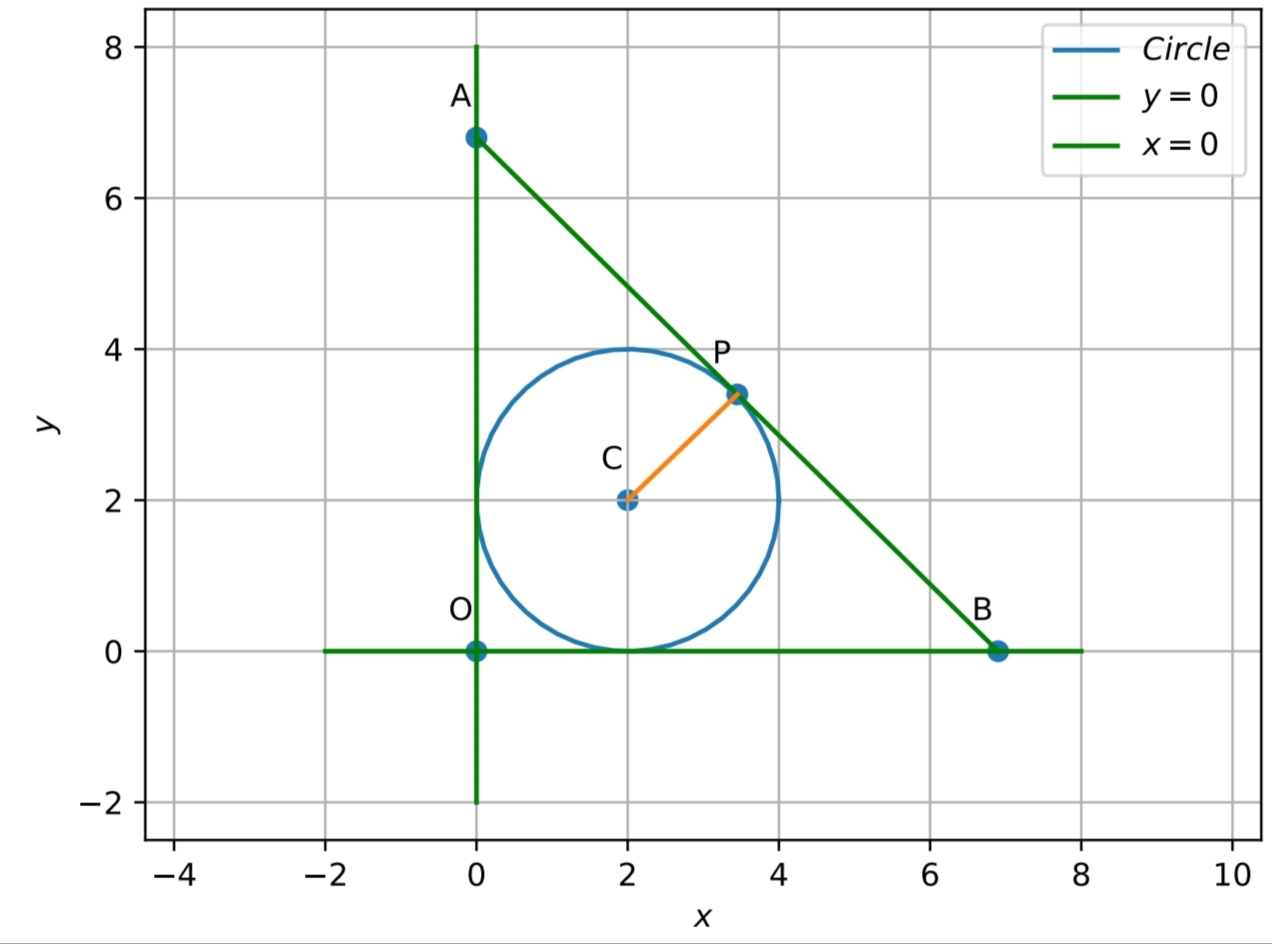
\includegraphics[scale=0.2]{cir.jpg}}\vspace{2mm}\\
\centering{Figure}\vspace{2mm}\\
	\vspace{10mm}
	\centering \large\textsc{3  C}\footnotesize\textsc{ONSTRUCTION}\vspace{5mm}\\
\raggedright\large{The circle and triangle are constructed with,} 
\begin{center}
    \label{tab:truthtable}
    \setlength{\arrayrulewidth}{0.2mm}
\setlength{\tabcolsep}{5pt}
\renewcommand{\arraystretch}{1.25}
    \begin{tabular}{|c|c|c|}
    \hline % <-- Alignments: 1st column left, 2nd middle and 3rd right, with vertical lines in between
      \large\textbf{Symbol} & \large\textbf{Co-ordinates} & \large\textbf{Description}\\
      \hline
       \large r& 2 & \large{radius}\\
       \large C & $\ \begin{pmatrix} 2\\ 2 \end{pmatrix}$ & center of the circle \\
       \large O & $\ \begin{pmatrix} 0\\ 0 \end{pmatrix}$ & origin\\
	
	\large A & $\ \begin{pmatrix} 0\\ b \end{pmatrix}$ &\makecell {point of intersection \\ with the Y-axis } \\
	\large B & $\ \begin{pmatrix} 0\\ a \end{pmatrix}$ &\makecell {point of intersection \\ with the X-axis}\\
	\large \textbf P & $\frac{A+B}{2} $ & circumcenter\\
      \hline
   \end{tabular}
 \end{center}\vspace{5mm}
\raggedright\large{The figure above is generated using python code provided in the below source code link.}\vspace{2mm}\\
\begin{mdframed}
\raggedright\large{https://github.com/sivagayathri \\ /FWC/blob/main/matrices/circles/cir.py}
\end{mdframed}
\end{multicols}
\end{document}
